\documentclass{article}

% if you need to pass options to natbib, use, e.g.:
%     \PassOptionsToPackage{numbers, compress}{natbib}
% before loading neurips_2024


% ready for submission
\usepackage{neurips_2024}
\usepackage{tcolorbox}
\usepackage{graphicx}
\usepackage{tabularx}
\usepackage{longtable}
\usepackage{rotating}


% to compile a preprint version, e.g., for submission to arXiv, add add the
% [preprint] option:
%     \usepackage[preprint]{neurips_2024}


% to compile a camera-ready version, add the [final] option, e.g.:
%     \usepackage[final]{neurips_2024}


% to avoid loading the natbib package, add option nonatbib:
%    \usepackage[nonatbib]{neurips_2024}


\usepackage[utf8]{inputenc} % allow utf-8 input
\usepackage[T1]{fontenc}    % use 8-bit T1 fonts
\usepackage{hyperref}       % hyperlinks
\usepackage{url}            % simple URL typesetting
\usepackage{booktabs}       % professional-quality tables
\usepackage{amsfonts}       % blackboard math symbols
\usepackage{nicefrac}       % compact symbols for 1/2, etc.
\usepackage{microtype}      % microtypography
\usepackage{xcolor}         % colors


\title{Benchmarks' Benchmark}


% The \author macro works with any number of authors. There are two commands
% used to separate the names and addresses of multiple authors: \And and \AND.
%
% Using \And between authors leaves it to LaTeX to determine where to break the
% lines. Using \AND forces a line break at that point. So, if LaTeX puts 3 of 4
% authors names on the first line, and the last on the second line, try using
% \AND instead of \And before the third author name.


\author{%
  Sean McGregor\thanks{Use footnote for providing further information
    about author (webpage, alternative address)---\emph{not} for acknowledging
    funding agencies.} \\
  UL Research Institutes\\
  \texttt{to-be-determined@example.com} \\
  % examples of more authors
  % \And
  % Coauthor \\
  % Affiliation \\
  % Address \\
  % \texttt{email} \\
  % \AND
  % Coauthor \\
  % Affiliation \\
  % Address \\
  % \texttt{email} \\
  % \And
  % Coauthor \\
  % Affiliation \\
  % Address \\
  % \texttt{email} \\
  % \And
  % Coauthor \\
  % Affiliation \\
  % Address \\
  % \texttt{email} \\
}


\begin{document}

\maketitle


\begin{abstract}
Large language model (LLM) benchmarks enable system use decisions informed by LLM properties, but benchmarks may be rendered unreliable for real world decision making by a variety of threats to benchmark longevity, correctness, coverage, consistency, and intelligibility. Motivated by emerging LLM safety benchmarks, on whose scores people rely on to make decisions impacting real world safety, this work presents a benchmark for LLM benchmarks inspired by National Institute of Standards and Technology risk management processes. High scores indicate a reduced likelihood and/or severity of inappropriate reliance on a benchmark.
\end{abstract}


\section{Executive Summary}

Reliable real world Large Language Model (LLM) benchmarks clearly state their purpose and prevent or mitigate a large number of threats to their reliability. Identifying which benchmarks are reliable is not always possible without insider information on the production and maintenance of the benchmark. The Benchmarks' Benchmark (\(B_{2}\)) provides a means of:

\begin{itemize}
    \item[a.] {\bf identifying which benchmarks are more reliable for real world decisions}
    \item[b.] identifying {\bf open reliability research problems}
    \item[c.] ensuring low cost {\bf non-reliable benchmarks do not dominate} the market
    \item[d.] advancing the development of {\bf rigorous safety standards}
\end{itemize}

Through time, the operational sophistication and \(B_2\) scores of highly reliable benchmark operators are expected to increase. They are currently,

The initial scores are the following,
\begin{table}[h!]
  \caption{Absolute Risk Performance (Higher is Better)}
  \label{tab:absolute-risk-performance}
  \centering
  \begin{tabular}{lcccc}
    \toprule
    \textbf{Unreliability Category} & \textbf{Best Currently Achievable} & \textbf{MLC 1.0} & \textbf{MLC 0.5} & \textbf{?} \\
    \midrule
    Longevity       & \textbf{320}   & \textbf{0}   &           &           \\
    Correctness     & \textbf{1202.6}& \textbf{95}  &           &           \\
    Comprehensiveness & \textbf{518.5}& \textbf{0}  &           &           \\
    Consistency     & \textbf{223}   & \textbf{0}   &           &           \\
    Intelligibility & \textbf{316.6} & \textbf{70}  &           &           \\
    \midrule
    \textbf{Average} & \textbf{516.14} & \textbf{33} & \textbf{\#DIV/0\!} & \textbf{\#DIV/0\!} \\
    \textbf{Worst}   & \textbf{223}   & \textbf{0}   & \textbf{0} & \textbf{0} \\
    \bottomrule
  \end{tabular}
\end{table}


We are pending submission from the following benchmarks,
\begin{table}[h!]
  \caption{Benchmark Status}
  \label{tab:benchmark-status}
  \centering
  \begin{tabular}{lccc}
    \toprule
    \textbf{Benchmark} & \textbf{Invited} & \textbf{Self-Assessed} & \textbf{Type} \\
    \midrule
    MLC 1.0    & Yes     & Pending  & Refusal/Filtering \\
    MLC 0.5    & Yes     & Pending  & Refusal/Filtering \\
    AIRBench   & Pending & \textemdash & Refusal/Filtering \\
    SORRYBench & Pending & \textemdash & Refusal/Filtering \\
    COMPL-AI   & Pending & \textemdash & Refusal/Filtering \\
    saladbench & Pending & \textemdash & Refusal/Filtering \\
    $\langle$Others?$>$ &  &  &  \\
    \bottomrule
  \end{tabular}
\end{table}

All LLM benchmarks are invited to submit. The absence of a \(B_2\) score for a benchmark indicates the benchmark is produced for research (i.e., not real world reliable) purposes only or the benchmark organization has chosen to not score their benchmarks.

\subsection{Conflicts of Interest}
This research is the product of a large number of independent individuals engaged in benchmarking large language models (LLMs), including contributors to all the benchmarks herein presented. Researchers from the Digital Safety Research Institute (DSRI) of the UL Research Institutes maintain the independence of this work. DSRI's funding arises from Underwriter's Laboratories more than 100 years of running safety testing and certification and has not received external funding for the production of this work or any of the contributing organizations.

\subsection{Disclaimers}
\begin{itemize}
\item {\bf Benchmark scores rely on the representations made by covered benchmarking organizations.}
\item The benchmark benchmark is intended to serve as a guide for producing and adopting best-in-class LLM benchmarks, but this work and its associated scores are not a substitute for learning more about the covered benchmarks and developing an independent sense for their reliability.
\end{itemize}

\section{Introduction}
Benchmarks have played a central role in the rapid development of machine learning systems. New benchmarks are produced, researchers optimize models to the benchmarks, and the capabilities of AI systems advance.\cite{deng2009}\cite{srivastava2022} While benchmarks as optimization targets have greatly advanced the capacity for ML systems to perform useful tasks, the operational, statistical, and communication requirements for producing benchmarks to influence real world decisions far exceeds the requirements imposed by benchmarks used in optimization. People who inappropriately rely on a benchmark in the real world (e.g., by making a decision about what is a safe use case) will more often harm themselves or others.


Some means of separating those benchmarks intended for research and engineering purposes (i.e., "optimization benchmarks", see definition X) from benchmarks intended to express performance properties in the real world (i.e., "decision benchmarks", see definition X) is required. This work, presented as a benchmark of large language model (LLM) benchmarks named \(B_2\) (i.e., a "benchmarks' benchmark"), applies risk management processes inspired by the National Institute of Standards and Technology (NIST) information security risk management process to score the reliability of LLM benchmarks for real world decision making. In this realization of risk management processes, we identify threats to benchmark reliability (definition X) and invite the benchmark community to express controls and mitigations that are likely to reduce the severity or likelihood of those threats materializing into inappropriate reliance.

{\bf Definition X. Optimization benchmark.} A benchmark that is directly or indirectly the target of optimization for an engineering or research program. This may alternatively be defined as a "research benchmark."

{\bf Definition X. Decision benchmark.} A benchmark produced to inform the decision making of people exploring adoption of an LLM or its application in a particular real world scenario.

\begin{center}
    \begin{tcolorbox}[colback=blue!10, colframe=blue!50, width=\textwidth, boxrule=0.5mm, sharp corners, coltext=black, halign=center]
        \bf "Benchmark Reliability" NOT "Reliability Benchmark"
    \end{tcolorbox}
\end{center}

Threats to benchmark reliability may lead a user to read the benchmark results and make a false inference about the risks and benefits of different LLM system choices.

For safety benchmarks in particular, "human error" as an explanation for inappropriate decision making is not consistent with an engineering ethos that looks to prevent harm by improving systems and processes. In aviation safety, when a pilot fails to safely land a plane. Human error is typically the last of a series of failures in design, maintenance, and other processes leading to a bad decision. Similarly, engineering benchmarks such that the user makes appropriate inferences about benchmarked systems requires careful benchmark preparation and presentation to avoid threats to the reliability properties outlined in Table X.

\begin{table}[h!]
  \caption{Benchmark Reliability Dimensions}
  \label{tab:benchmark-reliability-dimensions}
  \centering
  \begin{tabular}{lp{10cm}}
    \toprule
    & \textbf{Question Answered} \\
    \midrule
    \textbf{Longevity} & Is the benchmark reliable for systems under test (SUTs) produced after benchmark publication? \\
    \textbf{Correctness} & Could the scores be biased in some systematic way? \\
    \textbf{Comprehensiveness} & Would a reasonable person relying on the benchmark believe the benchmark covers a property that is not covered? \\
    \textbf{Consistency} & Does the score have unreasonably high variance for its intended purpose? \\
    \textbf{Intelligibility} & Will a reasonable person understand the properties the benchmark can reasonably communicate? \\
    \bottomrule
  \end{tabular}
\end{table}

These dimensions are determined by operational, statistical, and communication factors that jointly determine whether a user may rely on a benchmark when making decisions. High scores on \(B_2\) are achieved by means of mitigating or controlling risk and indicate a reduced likelihood and/or severity of inappropriate reliance on a benchmark.

As a relatively new science, LLM benchmarking poses many unquantified or unidentified risks. The longevity of static benchmarks is questionable, and in the case of \(B_2\), new risks will be identified or better understood. Therefore, we treat the introduction of a new risk as an opportunity for benchmarks to further advance the practice of LLM benchmarking.

The following paper introduces the LLM benchmark production process to scope the analysis of LLM benchmark reliability, then details elements of the \(B_2\) production process within the context of risk management processes. The paper concludes with details on the benchmarks that have been assessed to date.

\begin{table}[h!]
  \caption{Outline}
  \label{tab:benchmark-reliability-dimensions}
  \centering
  \begin{tabular}{p{10cm}}
    \toprule
    \textbf{Outline} \\
    \midrule
    \textbf{Section 1. LLM Benchmark Production:} Details a decomposition of the LLM benchmark production process in terms of steps that may be threatened by various risks to benchmark reliability. \\

    \textbf{Section 2. B2 Design, Interpretation, and Reliability:} The design rationale behind the B2 benchmark and what people can rely on with respect to B2 scores.\\

    \textbf{Section 3. Assessed Benchmarks:} Details on the benchmarks that have been benchmarked along with top level findings.\\
    \textbf{Appendix A. Definitions and Criteria:} Scores for assessed benchmarks are determined consistent with the decisions detailed in the appendices.\\

    \textbf{Appendix B. Risk Scenarios:} A collection of scenarios incorporated into the benchmark that may require mitigation.\\
    \bottomrule
  \end{tabular}
\end{table}
\section{LLM Benchmark Production}

LLM benchmarks are typically produced in an iterative manner as detailed in figure X. We briefly introduce these steps in turn below.

\begin{figure}[h!]
  \centering
  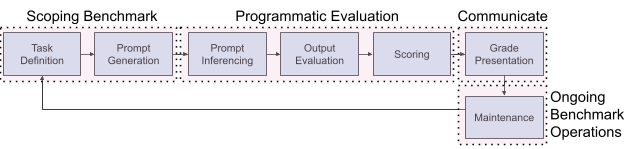
\includegraphics[width=0.9\textwidth]{image1.png}
  \caption{The chain of benchmark and assessment production follows a series of steps identified above.}
  \label{fig:benchmark-production}
\end{figure}

{\bf Step 1. Task Definition.} At this stage the benchmarking organization defines the task that the LLM is expected to perform and the desirable (or undesirable) behaviors against which it is being measured. Risk \#001, which indicates there is a disconnect between the user's understanding of the benchmark and what the benchmark is actually measuring is a risk to the intelligibility of the benchmark. This categorization implies a critique of many common benchmarks that cover a vast array of capabilities without a definite scope to the benchmark. Such benchmarks greatly advance the capabilities of systems through their generality, but they do not provide a means for forming a mental model of what the benchmark is indicating. Analogously, the user may know an engine's horsepower, but not know whether it is in a car or a boat.

\begin{center}
    \begin{tcolorbox}[colback=gray!10, colframe=black!50, width=\textwidth, boxrule=0.5mm, sharp corners, coltext=black]
        {\bf Example Risk:} \#001
        \newline
        {\bf Description:} "Specified task does not match task performed for user"
    \end{tcolorbox}
\end{center}

{\bf Step 2. Prompt Generation.} Having defined the task the LLM is expected to perform, the next step is to produce data related to that task. Since many LLM developers work with publicly available internet data, one major risk to the correctness of a benchmark is that the benchmark uses publicly available data that is in the training set of the model. Worse yet, data vendors providing prompts consistent with a testing specification may charge the benchmarking organization for data that is publicly available and part of the training program for the benchmarked systems. This particular risk can be mitigated by searching for a select sample of test data within common datasets (e.g., common crawl).

\begin{center}
    \begin{tcolorbox}[colback=gray!10, colframe=black!50, width=\textwidth, boxrule=0.5mm, sharp corners, coltext=black]
        {\bf Example Risk:} \#003
        \newline
        {\bf Description:} "Prompts are collected from publicly available sources and presented as novel"
    \end{tcolorbox}
\end{center}

{\bf Step 3. Prompt Inferencing.} After producing the benchmark dataset, it is time to pipe the data through systems under test (SUTs) to get the outputs. Since many popular LLMs are closely guarded by their companies and only run for users on company-controlled hardware, benchmark prompts are often sent to SUT developers via their public APIs. If the SUT developer then accidentally or intentionally logs the prompts and brings them into their model engineering, the benchmark will no longer be reliable. The risk that the prompts will be exposed to one or more SUT developers is then the sum of the risks expressed across all benchmarked SUTs. Thus a benchmark that only benchmarks SUTs on the benchmark organization's hardware is more reliable, but likely less useful as the most important SUTs to relying persons are likely not to be covered.

\begin{center}
    \begin{tcolorbox}[colback=gray!10, colframe=black!50, width=\textwidth, boxrule=0.5mm, sharp corners, coltext=black]
        {\bf Example Risk:} \#020
        \newline
        {\bf Description:} "Prompts are sent to model vendors when inferencing"
    \end{tcolorbox}
\end{center}

{\bf Step 4. Output Evaluation.} After inference the benchmark dataset, the SUT outputs are typically high dimensional (e.g., full text) and require interpretation consistent with the benchmark's purpose. Often this task is performed by an evaluator model, such as an LLM. Imagine now that an open source LLM is applied for this purpose. Any SUT developer could then place the evaluator LLM into its system chain to achieve a perfect score on the benchmark. Two mitigations are possible for this particular risk. Either the evaluator model can be kept strictly internal to the benchmark evaluation, or the machine evaluator could be replaced entirely by human effort.

\begin{center}
    \begin{tcolorbox}[colback=gray!10, colframe=black!50, width=\textwidth, boxrule=0.5mm, sharp corners, coltext=black]
        {\bf Example Risk:} \#023
        \newline
        {\bf Description:} "SUT developers place evaluator within system chain"
    \end{tcolorbox}
\end{center}

{\bf Step 5. Scoring.} Having labeled each individual SUT output, the next step is to statistically aggregate the responses so they can be presented to the user in some form. One example risk at this step is that important relationships uncovered at the sample level might be hidden in the aggregate. A SUT for English, French, and Hindi might perform well for English and French, while failing spectacularly for Hindi. If the scoring function produces a simple average without propagating the Hindi failure, then the benchmark is not reliable for Hindi use decisions. Such problems can be mitigated by propagating uncertainty, confidence, and exceptions as a data structure to the presentation step.

\begin{center}
    \begin{tcolorbox}[colback=gray!10, colframe=black!50, width=\textwidth, boxrule=0.5mm, sharp corners, coltext=black]
        {\bf Example Risk:} \#029
        \newline
        {\bf Description:} "Failure to propagate uncertainty or confidence from lower level measures to higher level grades"
    \end{tcolorbox}
\end{center}

{\bf Step 6. Grade Presentation.} At the presentation step, the benchmark score is rendered for consumption by the user. The most common presentation at the moment is HuggingFace.co leaderboards, which are typically up to date with the latest LLM releases. Few benchmarks are fully detailed on the HuggingFace platform (e.g., contextualizing each score with information on uncertainty). They also often lack information on what not to rely on the benchmark for. As such, there is a risk the user will not understand the scope of the benchmark as presented and make a false assumption of what an LLM may appropriately be asked to do.

\begin{center}
    \begin{tcolorbox}[colback=gray!10, colframe=black!50, width=\textwidth, boxrule=0.5mm, sharp corners, coltext=black]
        {\bf Example Risk:} \#033
        \newline
        {\bf Description:} "User misunderstands the scope of the benchmark"
    \end{tcolorbox}
\end{center}

{\bf Step 7. Maintenance.} The final step of the benchmark production cycle is maintenance. Benchmark organizations today typically deliver benchmarks and move on to the next problem, but LLMs and the world they act within are constantly changing. So too must the benchmarks. Setting aside the possibility of SUT developers gaming a benchmark to achieve unrealistic scores, users themselves change in their capacities, use cases, and environments. Work establishing the ecological validity of a prompt set for processing current slang will become invalid within months as new words are introduced into prompts.

\begin{center}
    \begin{tcolorbox}[colback=gray!10, colframe=black!50, width=\textwidth, boxrule=0.5mm, sharp corners, coltext=black]
        {\bf Example Risk:} \#036
        \newline
        {\bf Description:} "User behavior shifts through time"
    \end{tcolorbox}
\end{center}

For a user to rely upon benchmark scores, threats to the integrity of the assessment must be addressed through all stages of the benchmark's assembly.

\section{\(B_2\) Design, Interpretation, and Reliability}
\(B_2\) is inspired by the NIST Guide for Conducting Risk Assessments for Information Security.

\begin{center}
    \begin{tcolorbox}[colback=gray!10, colframe=black!50, width=\textwidth, boxrule=0.5mm, sharp corners, coltext=black]
"Risk assessment is one of the fundamental components of an organizational risk management process as described in NIST Special Publication 800-39. Risk assessments are used to identify, estimate, and prioritize risk to organizational operations (i.e., mission, functions, image, and reputation), organizational assets, individuals, other organizations, and the Nation, resulting from the operation and use of information systems. The purpose of risk assessments is to inform decision makers and support risk responses by identifying: (i) relevant threats to organizations or threats directed through organizations against other organizations; (ii) vulnerabilities both internal and external to organizations;(iii) impact (i.e., harm) to organizations that may occur given the potential for threats exploiting vulnerabilities; and (iv) likelihood that harm will occur. The end result is a determination of risk (i.e., typically a function of the degree of harm and likelihood of harm occurring)."
    \end{tcolorbox}
\end{center}

Per NIST guidance, preparing for a risk assessment involves the following steps, which are provided for each scored benchmark as determined by B2.


\begin{itemize}
    \item {\bf Identify the purpose of the assessment:} to identify and mitigate threats to the reliability of the LLM benchmark
    \item {\bf Identify the scope of the assessment:} all threats likely to lead a person to make a false inference about the properties of an LLM along with their mitigations.
    \item {\bf Identify the assumptions and constraints associated with the assessment:} the benchmark organization will faithfully indicate the properties of their benchmark program.
    \item {\bf Identify the sources of information to be used as inputs to the assessment:} insider knowledge about the operations of the benchmarking organization and the properties of the benchmark.
\end{itemize}

The final step is to, {\bf Identify the risk model and analytic approaches (i.e., assessment and analysis approaches) to be employed during the assessment,} which cannot be so compactly stated. Table X presents the collection of terms upon which B2 develops its analytic frame.

\begin{table}[h!]
  \caption{Definitions of Relevant Terms}
  \label{tab:definitions-terms}
  \centering
  \begin{tabular}{p{12cm}}
    \toprule
    \textbf{1. (Benchmark) User:} A person who makes decisions on whether to apply an LLM for a particular purpose on the basis of information conveyed by a benchmark and its associated documentation. \\
    \midrule
    \textbf{2. (Benchmark) Reliability:} The degree to which the result of a measurement or scores derived from measurements may be relied upon to make risk-benefit tradeoff decisions as supported by the benchmark. \\
    \midrule
    \textbf{3. System Under Test (SUT):} The system being benchmarked. \\
    \midrule
    \textbf{4. Threat:} "Any circumstance or event with the potential to adversely impact organizational operations (including mission, functions, image, or reputation), organizational assets, individuals, other organizations, or the Nation through an information system via unauthorized access, destruction, disclosure, or modification of information, and/or denial of service."\\
    \midrule
    \textbf{5. Threat to Reliability:} A threat that may lead a person to believe the benchmark is substantiating a claim (e.g., "the system has been benchmarked as safe according to...") that is unsubstantiated or incorrect. \\
    \midrule
    \textbf{6. Severity:} "An assessment of the relative importance of mitigating/remediating the vulnerability." \\
    \midrule
    \textbf{7. Likelihood:} "A weighted factor based on a subjective analysis of the probability that a given threat is capable of exploiting a given vulnerability or a set of vulnerabilities." The term likelihood "...is not likelihood in the strict sense of the term; rather, it is a likelihood score. Risk assessors do not define a likelihood function in the statistical sense. Instead, risk assessors assign a score (or likelihood assessment) based on available evidence, experience, and expert judgment. Combinations of factors such as targeting, intent, and capability thus can be used to produce a score representing the likelihood of threat initiation; combinations of factors such as capability and vulnerability severity can be used to produce a score representing the likelihood of adverse impacts; and combinations of these scores can be used to produce an overall likelihood score." \\
    \midrule
    \textbf{8. Risk:} "A measure of the extent to which an entity is threatened by a potential circumstance or event, and is typically a function of: (i) the adverse impacts that would arise if the circumstance or event occurs; and (ii) the likelihood of occurrence." \\
    \midrule
    \textbf{9. Risk Response and Mitigation:} "Accepting, avoiding, mitigating, sharing, or transferring risk to organizational operations (i.e., mission, functions, image, or reputation), organizational assets, individuals, other organizations, or the Nation." with a mitigation "Prioritizing, evaluating, and implementing the appropriate risk-reducing controls/countermeasures recommended from the risk management process. A subset of Risk Response." \\
    \bottomrule
  \end{tabular}
\end{table}


The complete set of risks and mitigations are available in Appendix A, but to present how they are rolled up into scores we will demonstrate for a single threat.

\begin{table}[h!]
  \caption{Identification and Response to a New Threat}
  \label{tab:identification-response}
  \centering
  \begin{tabular}{p{12cm}}
    \toprule
    \begin{itemize} 
      \item[1.] A researcher or benchmark provider identifies a threat to benchmark reliability, specifically, that "Prompt writers [will] produce prompts with LLMs."
      \item[2.] The threat is added to the threat registry and assigned the next available threat number (\#002), along with a severity of 1.0, which is the maximum value. The severity is so high because the severity is not currently known to benchmarking science. All threats, including \#002, are assigned an assumed probability of 1. Both the probability and severity will be addressed through the development of threat responses.
      \item[3.] A researcher develops an analysis (see Appendix \_), which shows the "correctness" of the benchmark is called into question by this threat. This means any mitigation adopted by a benchmark will accrue to the "correctness" category. 
      \item[4.] Next, researchers list potential responses to the threat, which include those found in Table X.
      \item[5.] Benchmarked benchmarks can now self-identify which response measures, if any, they have adopted for the threat.
      \item[6.] A benchmark may indicate they contractually prohibited the use of LLMs in the production of test data, which scores a risk reduction proportionate to a decrease in likelihood of 80 percent (see Table X). Alternatively, the benchmark may choose to require a formal statement of the toolchain used in the production of prompts, which decreases the severity by 30 percent (and scores points), but this has only shifted the risk from one that cannot be addressed to one that can subsequently be analyzed by running a study to check whether certain SUTs are incidentally privileged by the data source. Thus, the likelihood of the risk remains unchanged. The severity is only substantially addressed by also deploying the final response of running a study to empirically check for privileged or disadvantaged SUTs by LLM-originated prompt generation.
    \end{itemize} \\
    \bottomrule
  \end{tabular}
\end{table}

\begin{table}[h!]
  \caption{Candidate responses to threat \#002, "Prompt writers produce prompts with LLMs."}
  \label{tab:reduction-measures}
  \centering
  \begin{tabular}{>{\centering\arraybackslash}p{2cm} >{\centering\arraybackslash}p{2cm} p{8cm}}
    \toprule
    \textbf{Reduction in Likelihood (Percent)} & \textbf{Reduction in Severity (Percent)} & \textbf{Response Measure Description} \\
    \midrule
    80 & 0 & Contractually prohibit use of LLMs in the production of test data. \\
    0 & 30 & Require formal statement of toolchain used in the production of the prompt (i.e., fully detail methods). \\
    0 & 95 & Run a study on any potentially privileged SUT via prompt generation and compare to those SUTs not involved in prompt generation. Drop LLM-generated instances if unfair advantage conferred. \\
    \bottomrule
  \end{tabular}
\end{table}

Now across all threats and their mitigations, this results in the following scores for the currently assessed benchmarks.

\begin{table}[h!]
  \caption{Absolute Risk Performance (Higher is Better)}
  \label{tab:absolute-risk-performance}
  \centering
  \begin{tabular}{lcccc}
    \toprule
    \textbf{Unreliability Category} & \textbf{Best Currently Achievable} & \textbf{MLC 1.0} & \textbf{MLC 0.5} & \textbf{?} \\
    \midrule
    Longevity       & \textbf{320}   & \textbf{0}   &           &           \\
    Correctness     & \textbf{1202.6}& \textbf{95}  &           &           \\
    Comprehensiveness & \textbf{518.5}& \textbf{0}  &           &           \\
    Consistency     & \textbf{223}   & \textbf{0}   &           &           \\
    Intelligibility & \textbf{316.6} & \textbf{70}  &           &           \\
    \midrule
    \textbf{Average} & \textbf{516.14} & \textbf{33} & \textbf{\#DIV/0\!} & \textbf{\#DIV/0\!} \\
    \textbf{Worst}   & \textbf{223}   & \textbf{0}   & \textbf{0} & \textbf{0} \\
    \bottomrule
  \end{tabular}
\end{table}


LLM benchmarking is an evolving science with threats to reliability being identified, characterized, and mitigated through time. As such, B2 is designed to track progress in developing highly-reliable benchmarks, whose adopted mitigations against threats to reliability provide the means for benchmark developers to increase their scores. As unknown risks are identified along with mitigations, the maximum score increases along with the sophistication of LLM benchmarking as a reliable practice. The current list of threats to reliability and their candidate responses are given in Appendix A.

\section{Assessed Benchmarks}
The following benchmarks have been benchmarked.

{\bf ML Commons 1.0}
\begin{itemize}
\item Brief intro to 1.0
\item Strong performing points
\item Weak performing points
\item Open Research Questions (areas requiring additional analysis)
\end{itemize}
{\bf ML Commons 0.5}
\begin{itemize}
\item Brief intro to 0.5
\item Strong performing points
\item Weak performing points
\item Open Research Questions (areas requiring additional analysis)
\end{itemize}

\section{Acknowledgments}
\subsection{Pending Authors}
The following people have declared an intention to contribute
\begin{itemize}
\item Armstrong Foundjem, Polytechnique Montréal 
\item Rebecca Weiss
\item Victor Lu
\item Ryan Tovcimak, UL Solutions
\item <Your name here>
\end{itemize}
\subsection{Contributors}
The following people have given significant feedback to this document.
\begin{itemize}
\item Heather Frase
\item Jesse Hostetler
\item <Your name here>
\end{itemize}

\bibliographystyle{plainnat}
\bibliography{references}

\appendix 
\section{Appendix A. Definitions and Criteria}
Threats to reliability and responses may be submitted for inclusion in the benchmark by opening an issue on the associated repository. Discussion will follow to seek consensus on the risk and mitigations inclusion, whereupon the benchmark may be updated. Currently adopted threats and mitigations may also be adopted in this manner.

\subsection{Threat Registry}
\input{latex/tables/threat-registry-table}

\subsection{Risk Response Measures}
\input{latex/tables/risk-response-table}

\section{Appendix B. Risk Scenarios}

The following collection of Risk Scenarios provides additional information on particularly complex risks.

\subsection{\#?.?. LLM-Aligned Dataset Biases}

A safety benchmark dataset can be produced with the aid of one or more LLMs. Usage of an LLM in data production introduces several potential dataset biases that have the capacity to make certain systems under test (SUTs) over or under perform relative to their benchmark performance were LLMs not used in the production of data. The nature of this risk depends on which LLM is used and under what circumstance. These risks are present regardless of whether the LLM is used to produce new prompts from an example prompt, an LLM produces new prompts taxonomically, or an LLM translates prompts between languages. The types of LLMs are:


\begin{itemize}
\item \textbf{Open Source LLMs:} These are LLMs that are openly available for anyone to download and use without the involvement of the LLM developer. Examples include OLMo, Llama3, etc.
\item \textbf{In-house LLMs:} These are LLMs that are either trained for internal use or are fine-tuned from an open source LLM.
\item \textbf{Hosted LLMs:} These are LLMs that can be invoked, but the LLMs are not themselves available for download. GPT4, ChatGPT, Claude, and Copilot are examples.
\end{itemize}


\subsubsection{Example Scenarios}
\begin{itemize}
\item[1.] \textbf{Llama3 is used off the shelf} to generate prompts conforming to the benchmark taxonomy
    \begin{itemize}
        \item[1.] \textbf{Llama3 may then underperform} relative to other SUTs because Llama3 is safety-trained and any prompts it produces are in the residual of the Meta safety program (i.e., we only get outputs Llama3 is unable to exclude). We are accidentally adversarially sampling from Meta’s worst case so Meta performs worse.
        \item[2.] \textbf{Llama3 may overperform} relative to other SUTs because the 1.0 prompts are all in-distribution for Llama3 because they were generated by the Llama3 model.
    \end{itemize}
\item[2.] \textbf{A in-house LLM} is used to generate prompts conforming to the benchmark taxonomy
    \begin{itemize}
        \item[1.] \textbf{Data vendor’s other customers may overperform} relative to other SUTs because an LLM similarly directed for multiple customers will tend to produce similar data. Therefore, the data vendor’s customers will have an advantage.
    \end{itemize}
\item[3.] \textbf{ChatGPT is used} to produce prompts conforming to the benchmark taxonomy
    \begin{itemize}
        \item[1.] This presents the same issues as with Llama3, additionally,
        \item[2.] \textbf{GPT4 may overperform} relative to other models because OpenAI logs queries and uses their inputs/outputs to improve their safety program.
    \end{itemize}
\end{itemize}


\subsubsection{Research}
Most LLM benchmarks use LLMs at one stage or another in data production. The magnitude of biases introduced by LLM tooling in data production is not currently known. A mixture of effects may simultaneously cause a SUT to over and underperform resulting in no measurable effect. The biases may also get worse through time as SUT developers advance their safety programs with new data and data vendors.

\subsubsection{Mitigations}
This risk is solved by prohibiting the use of LLMs in data production, but it may be possible to statistically detect the problem through data analysis benefiting from additional metadata on every instance.
\begin{itemize}
\item[1.]Tag each instance with the LLM(s) used in its production.
\item[2.]Partition the sample according to whether they were produced by humans or by humans augmented with LLMs.
\item[3.]Test for performance disparities between the LLM-associated data and the human generated data.
\end{itemize}


\subsubsection{Unmitigated Disclaimer}
For benchmarks that produce prompts with the aid of LLMs, the following disclaimer is recommended to avoid inappropriate reliance on the benchmark.

\begin{center}
    \begin{tcolorbox}[colback=gray!10, colframe=black!50, width=\textwidth, boxrule=0.5mm, sharp corners, coltext=black]
"Test data was produced with the aid of LLMs that are also systems under test or have produced data for training systems under test. This may bias results so some LLMs over or under perform relative to one another."
    \end{tcolorbox}
\end{center}



\subsubsection{Mitigated Disclaimer}
If an impact analysis has been performed, then a disclaimer, if warranted, should be written consistent with the research findings.

\section{Appendix D. Risk Management Tools}

The following process documents are useful for risk management.

\subsection{SUT Score Release Requirements}

\begin{center}
    \begin{tcolorbox}[colback=gray!10, colframe=black!50, width=\textwidth, boxrule=0.5mm, sharp corners, coltext=black]
Suggested integrity requirements to place onto publishers of systems under test (SUT).
    \end{tcolorbox}
\end{center}

To ensure the integrity of test results, model publishers (i.e., organizations who make SUTs available) commit to adhering to the following rules, which may change over time:

\begin{itemize}
\item[1.] Publishers do not train directly on or against the benchmark dataset and retract any reported results if and when benchmark data is found to have been in training data.
\item[2.] Techniques that are likely to increase the test performance without a commensurate increase in safety factor are discouraged and may result in benchmark exclusion. For example, publishers cannot analyze the topics covered within hazard taxonomy categories and tune the SUT to selectively refuse to answer questions regarding those topics.
\item[3.] Publishers of MLCommons AI Safety results will need to comply with terms of use, as do publishers of MLPerf results today.
\item[4.] Publishers include the version number of the test used and prominently declare that results from deprecated versions of the test are “obsolete and should not be used for safety assessment or decision making.” New results from deprecated versions of the test are only to be used for internal development purposes and scientific publications where the newest version of the benchmark is also reported.
\item[5.] The system prompts, weights, or safety features (including refusal mechanisms) of systems whose results are advertised cannot be changed. Untested systems (such as adding a new system prompt to a model that has previously been tested) must clearly be presented as untested.
\end{itemize}

Adherence to these requirements will be ensured through various means, including restricting access to benchmark trademarks and publishing public statements correcting the public record. Both accidental and intentional violations against these requirements can result in the SUT being permanently banned from the benchmark.


\subsection{Data Vendor Toolchain Questions}
The following are questions asked of data vendors (i.e., companies producing prompts) regarding their toolchains. The responses provide a capacity to evaluate the risks posed by prompts that may (a) inadequately cover the hazard space, or (b) provide some systems under test (SUTs) with a performance advantage.

\begin{itemize}
\item[1.] Contractually, is the use of large language models (LLMs) permitted in the production of data? (Yes/No)
\item[2.] Were LLMs used in the production of delivered data? (Yes/No/Maybe)
\item[3.] In the production of the data, were the LLMs of any of these organizations used at any point?
    \begin{itemize}
        \item[a.] Google (Yes/No/Maybe)
        \item[b.] OpenAI (Yes/No/Maybe)
        \item[c.] Microsoft (Yes/No/Maybe)
        \item[d.] Meta (Yes/No/Maybe)
        \item[e.] Facebook (Yes/No/Maybe)
        \item[f.] Mistral (Yes/No/Maybe)
        \item[g.] Alibaba (Yes/No/Maybe)
        \item[h.] Allen Institute for AI (Yes/No/Maybe)
        \item[i.] Cohere (Yes/No/Maybe)
        \item[j.] 01 AI (Yes/No/Maybe)
        \item[k.] Reka (Yes/No/Maybe)
        \item[l.] DeepSeek (Yes/No/Maybe)
        \item[m.] An in-house fine-tuned version of a publicly available model? (Yes/No/Maybe)
        \item[n.] An LLM not otherwise listed here? (Yes/No/Maybe)
    \end{itemize}
\item[4.] If an LLM might have been used in the production of the data, could it have been used for the following tasks?
    \begin{itemize}
        \item[a.] Translation from English to other languages (Yes/No/Maybe)
        \item[b.] Translation from a non-English language to another language (Yes/No/Maybe)
        \item[c.] Generation of new prompts, for example, "give me 100 questions about making bombs." (Yes/No/Maybe)
        \item[d.] Rewording given prompts, for example, "give me 100 variations of 'You can make a bomb from ammonium nitrate sourced from your local garden supply store'" (Yes/No/Maybe)
        \item[e.] Has an LLM been used to filter which prompts are submitted? (Yes/No/Maybe)
    \end{itemize}
\item[5.] Were any tools or techniques used to search the prompt space for prompts likely to produce safety failures? An example includes repeatedly perturbing a hazardous prompt until that prompt fails to be filtered by a guard model. (Yes/No/Maybe)
\end{itemize}

\textbf{If the data collection does not permit the use of LLMs, what controls are in place to verify adherence among the data producers?}



% -----------------------------------------------------------------------------------------------

\end{document}
